\section*{Dati e risultati}

\subsection*{Filtro Passa-Basso}

Per ottenere un filtro Passa-basso, illustrato in Figura \ref{fig:basso}, abbiamo montato un circuito $R\,C$ con una resistenza in serie ad un condensatore.
La caratteristica di tale filtro è quella di permettere il passaggio di tutte le frequenze che spaziano tra i $0\,\si{\hertz}$ fino alla frequenza di taglio ($\nu\ped{0}$), caratteristica propria del circuito determinata dai componenti dello stesso.
In questa prima parte ci interessa verificare pertanto che tale circuito si comporti effettivamente come un filtro passa-basso.

Noi sappiamo che la frequenza di taglio è quella frequenza che impone ad un segnale in uscita da un circuito, rispetto a quello di entrata, uno sfasamento di $\frac{\pi}{4}$ o in altri termini un'attenuazione della sua intensità di $\frac{1}{\sqrt{2}}$.
Pertanto conoscendo la relazione che sussiste tra la frequenza di taglio ($\nu\ped{0}$), la resistenza ($R$) ed il codensatore ($C$):

\begin{equation}
	\nu\ped{0} \,=\, \frac{1}{2\,\pi\,R\,C}
	\label{eq:taglio basso}
\end{equation}
%
possiamo determinare il valore della frequenza di taglio imponendo un valore di resistenza e capacità a piacere. I valori stabiliti sono i seguenti:

\begin{equation*}
	\text{Frequenza di taglio:} \quad \nu\ped{0} \,=\, 795 \,\pm\, 11 \,\, \si{\hertz}
\end{equation*}
\begin{equation*}
	\text{Resistenza:} \quad R \,=\, 1000 \,\pm\, 10 \,\, \si{\ohm}
\end{equation*}
\begin{equation*}
	\text{Capacità:} \quad C \,=\, 200 \,\pm\, 2 \,\, \si{\nano\farad} 
\end{equation*}

Quindi una volta realizzato il circuito e note le sue caratteristiche abbiamo raccolto una serie di valori relativi alla tensione in ingresso al circuito ($V\ped{in}$), la tensione ai capi del condensatore ($V\ped{out}$) e la frequenza del segnale in uscita ($\nu\ped{out}$).
In questo modo potremo studiare la funzione di trasferimento del filtro al variare della frequanza in ingresso ($\nu\ped{in}$).

\begin{SCfigure}
  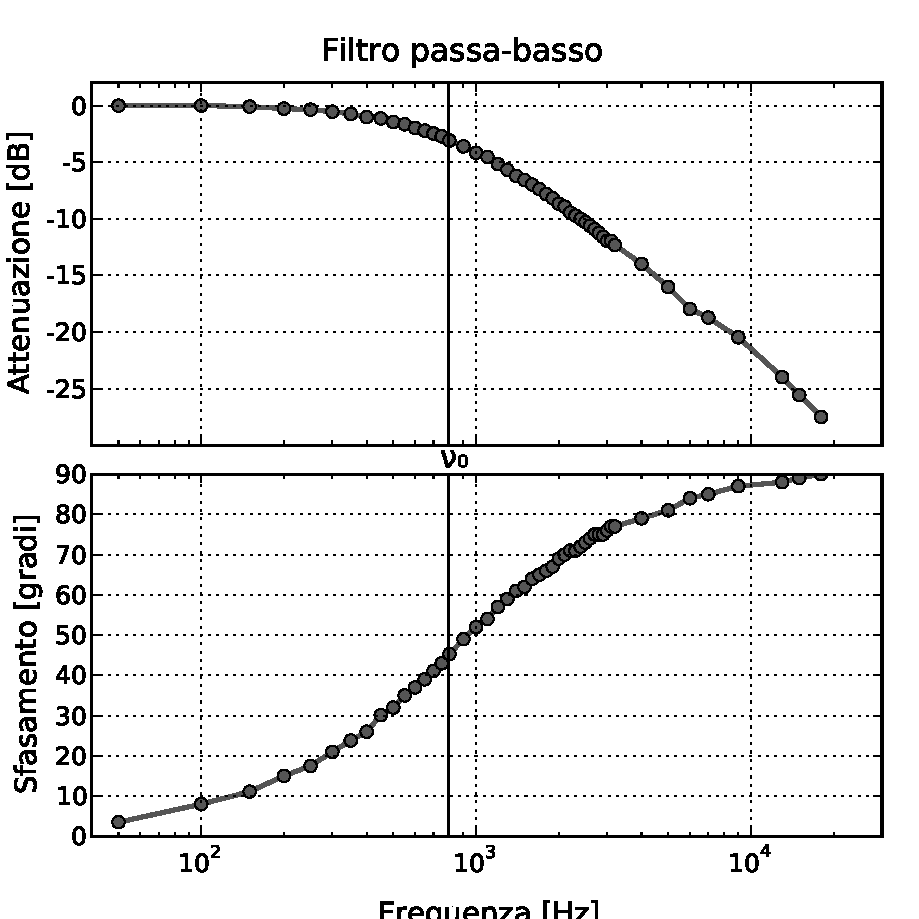
\includegraphics[scale=0.55]{passa_basso.pdf}
  \caption{I grafici riportano l'attenuazione e lo sfasamento tra input e output di un filtro passa-basso.
    Le curve grigie sono gli andamenti teorici, che sono molto bene seguiti dai dati sperimentali. Abbiamo
    scelto, come valore della frequenza di taglio, 800 Hz poiché avevamo a disposizione le capacità
    e resistenze adatte. In questo tipo di semplici filtri si ha un attenuazione, a frequenze più alte della
    frequenza ti taglio, che è di circa -20 dB/decade, o -6 dB/ottava. L'attenuazione risulta seguire questa
    ``regola'' dai nostri dati sperimentali. Inoltre si vede che a una decade di distanza dalla frequenza di taglio,
    lo sfasamento dista di meno di $6^\circ$ dai valori massimi e minimi, altra caratteristica tipica dei filtri RC.}
  \label{fig:g_basso}
\end{SCfigure}

\subsection*{Filtro Passa-Banda}


Per ottenere un filtro Passa-banda, illustrato in Figura \ref{fig:banda}, abbiamo montato un circuito $R\,C\,L$ con una resistenza in serie al parallelo tra un'induttanza ed un condensatore.
La caratteristica di tale filtro è quella di permettere il passaggio di frequenze che appartengono solo ad un determinato intervalo centrato intorno alla frequenza di risonanza ($\nu\ped{r}$), mentre atenua tutte quelle non appartenenti ad esso.
In questo caso a noi interessa ricavare, stabilita una certa frequenza di risonanza, l'intervallo di frequenze che vengono trasmesse e verificare pertato che tale circuito sia una buona approssimazione di un filtro passa-banda.

Poiche conosciamo la relazione che lega la frequenza di risonanza ($\nu\ped{r}$) con l'induttanza ($L$) e la capacità ($C$):

\begin{equation}
	\nu\ped{r} \,=\, \frac{1}{2\,\pi\,\sqrt{L\,C}}
	\label{eq:risonanza banda}
\end{equation}
%
\begin{wrapfigure}{r}{0.35\textwidth}
  \vspace{-0.5cm}
  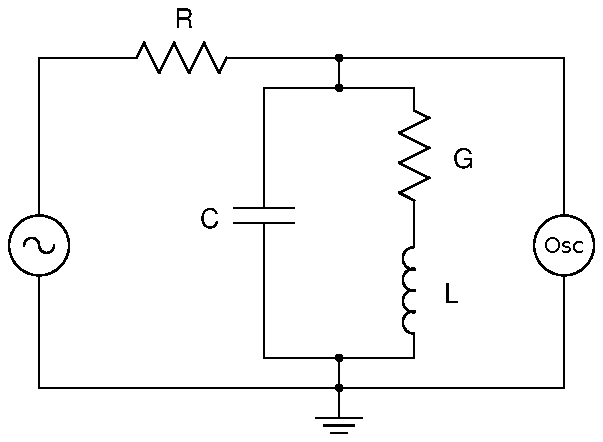
\includegraphics[width=0.33\textwidth]{s_corr2.pdf}
  \caption{Circuito corretto.}
  \label{fig:corr2}
  \vspace{-1.5cm}
\end{wrapfigure}
%
possiamo determinare il valore della frequnza di risonanza scegliendo a piacere i valori di induttanza e capacità. Pertanto la nostra scelta è stata la seguente:

\begin{align*}
	\text{Frequenza di risonanza:} \quad \nu\ped{r} \,=\, 10065 \,\pm\, 5 \, \si{\hertz} \\
	\text{Induttanza:} \quad L \,=\, (1.00 \,\pm\, 0.01)\cdot\,10^{-2} \, \si{\farad} \\
	\text{Capacità:} \quad C \,=\, 25 \,\pm\, 0.25 \, \si{\nano\farad} \\
\end{align*}

Quindi anche in questo caso raccoglindo, mediante l'oscilloscopio, una serie di valori relativi alla tensione in ingresso al circuito ($V\ped{in}$), la tensione ai capi del condensatore ($V\ped{out}$) e la frequenza del segnale in uscita ($\nu\ped{out}$), possiamo studiare la funzione di trasferimento del segnale al variare della frequanza in ingresso ($\nu\ped{in}$) al circuito.

\begin{SCfigure}
  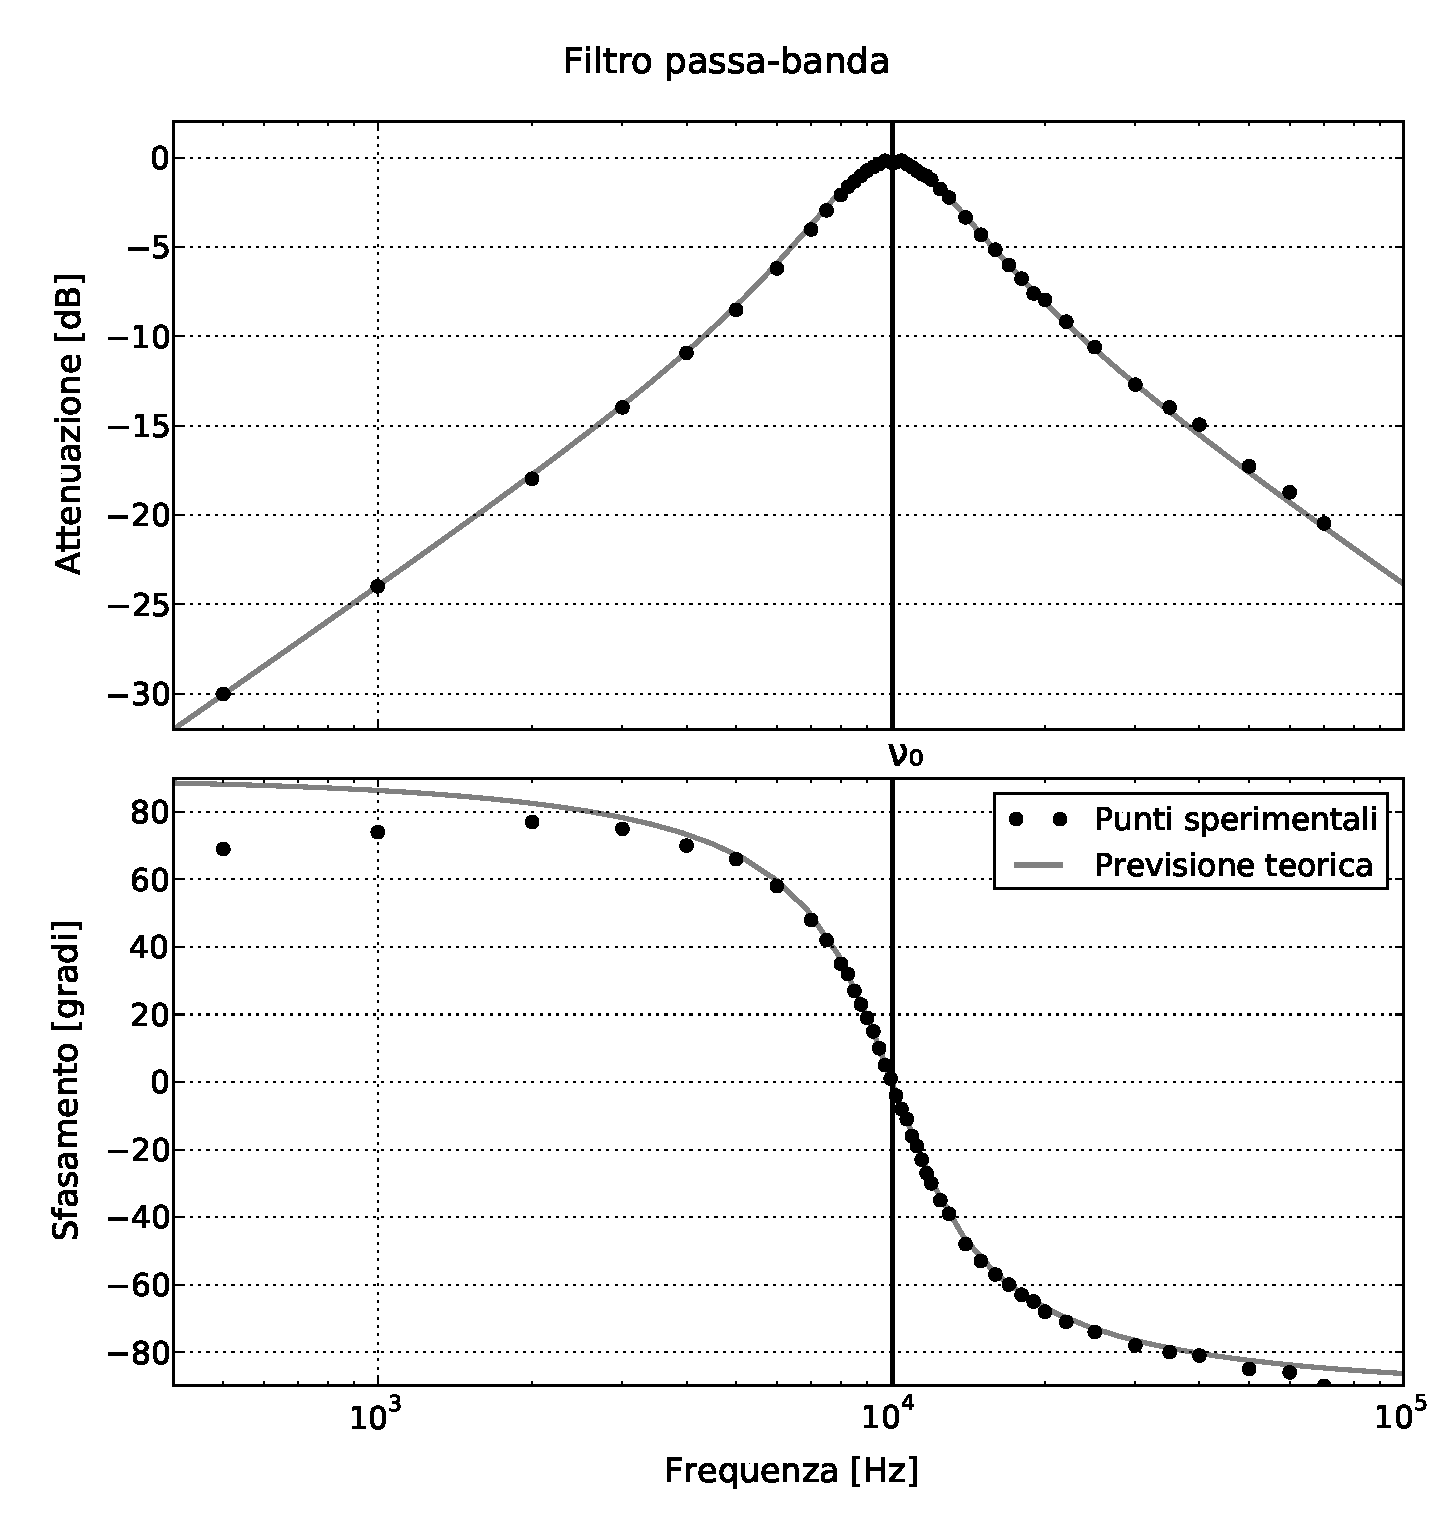
\includegraphics[scale=0.55]{passa_banda.pdf}
  \caption{Il primo grafico illustra l'attenuazione del segnale in funzione della frequenza del segnale stesso
    per un filtro passa-banda.
    Il secondo riporta lo sfasamento tra input e output, sempre in funzione della frequenza. La linea grigia indica
    gli andamenti delle due grandezze previsti dai calcoli. Il fattore di qualità vale
    $Q = \nu_0/\Delta \nu\ped{3dB} \simeq 1.4$ per il nostro filtro. I dati seguono bene la predizione teorica,
    unico neo i dati di sfasamento per basse frequenze. Per comprendere questa discrepanza abbiamo considerato una
    resistenza di valore $G = \SI{10}{\ohm}$ in serie all'induttanza, come mostrato in Figura \ref{fig:corr2},
    poiché un induttore reale ha anche una resistenza. La curva tratteggiata illustra l'andamento previsto dopo aver introdotto la
    correzione. Poichè tale curva segue molto bene i dati, possiamo concludere che la resistenza dell'induttore è
    la ragione della differenza tra dati e teoria.
    Le incertezze sono dell'ordine di grandezza dei punti ($\simeq 1\%$).}
  \label{fig:g_banda}
\end{SCfigure}

\subsection*{Filtro a Reiezione di Banda}

\begin{wrapfigure}{r}{0.35\textwidth}
  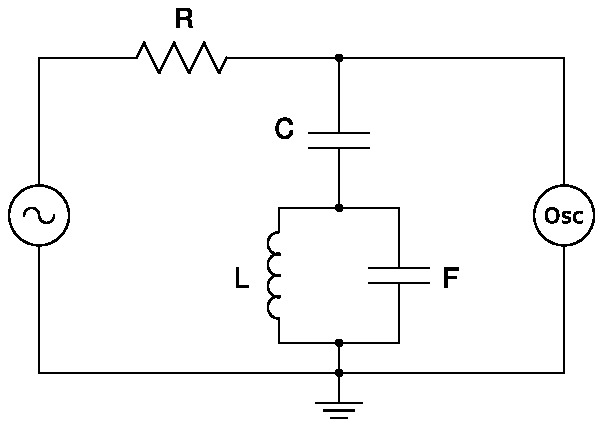
\includegraphics[width=0.33\textwidth]{s_corr.pdf}
  \caption{Circuito corretto.}
  \label{fig:corr}
\end{wrapfigure}

Per ottenere un filtro a Reiezione di banda, illustrato in Figura \ref{fig:notch}, abbiamo montato un circuito $R\,C\,L$ con una resistenza in serie ad un'induttanza ed un condensatore.
Questo filtro non è altro che l'opposo del filtro Passa-banda ovvero, nota la frequenza di risonanza ($\nu\ped{r}$), il filtro impedisce la trasmissione delle frequenze appartenenti all'intervallo centrato su $\nu\ped{r}$. L'analisi che viene fatta per questo circuito è del tutto analoga a quella illustrata per il filtro Passa-banda, come anche i valori di capacità, induttanza e frequenza di risonanza esposti nella sezione precedente.

\begin{SCfigure}
  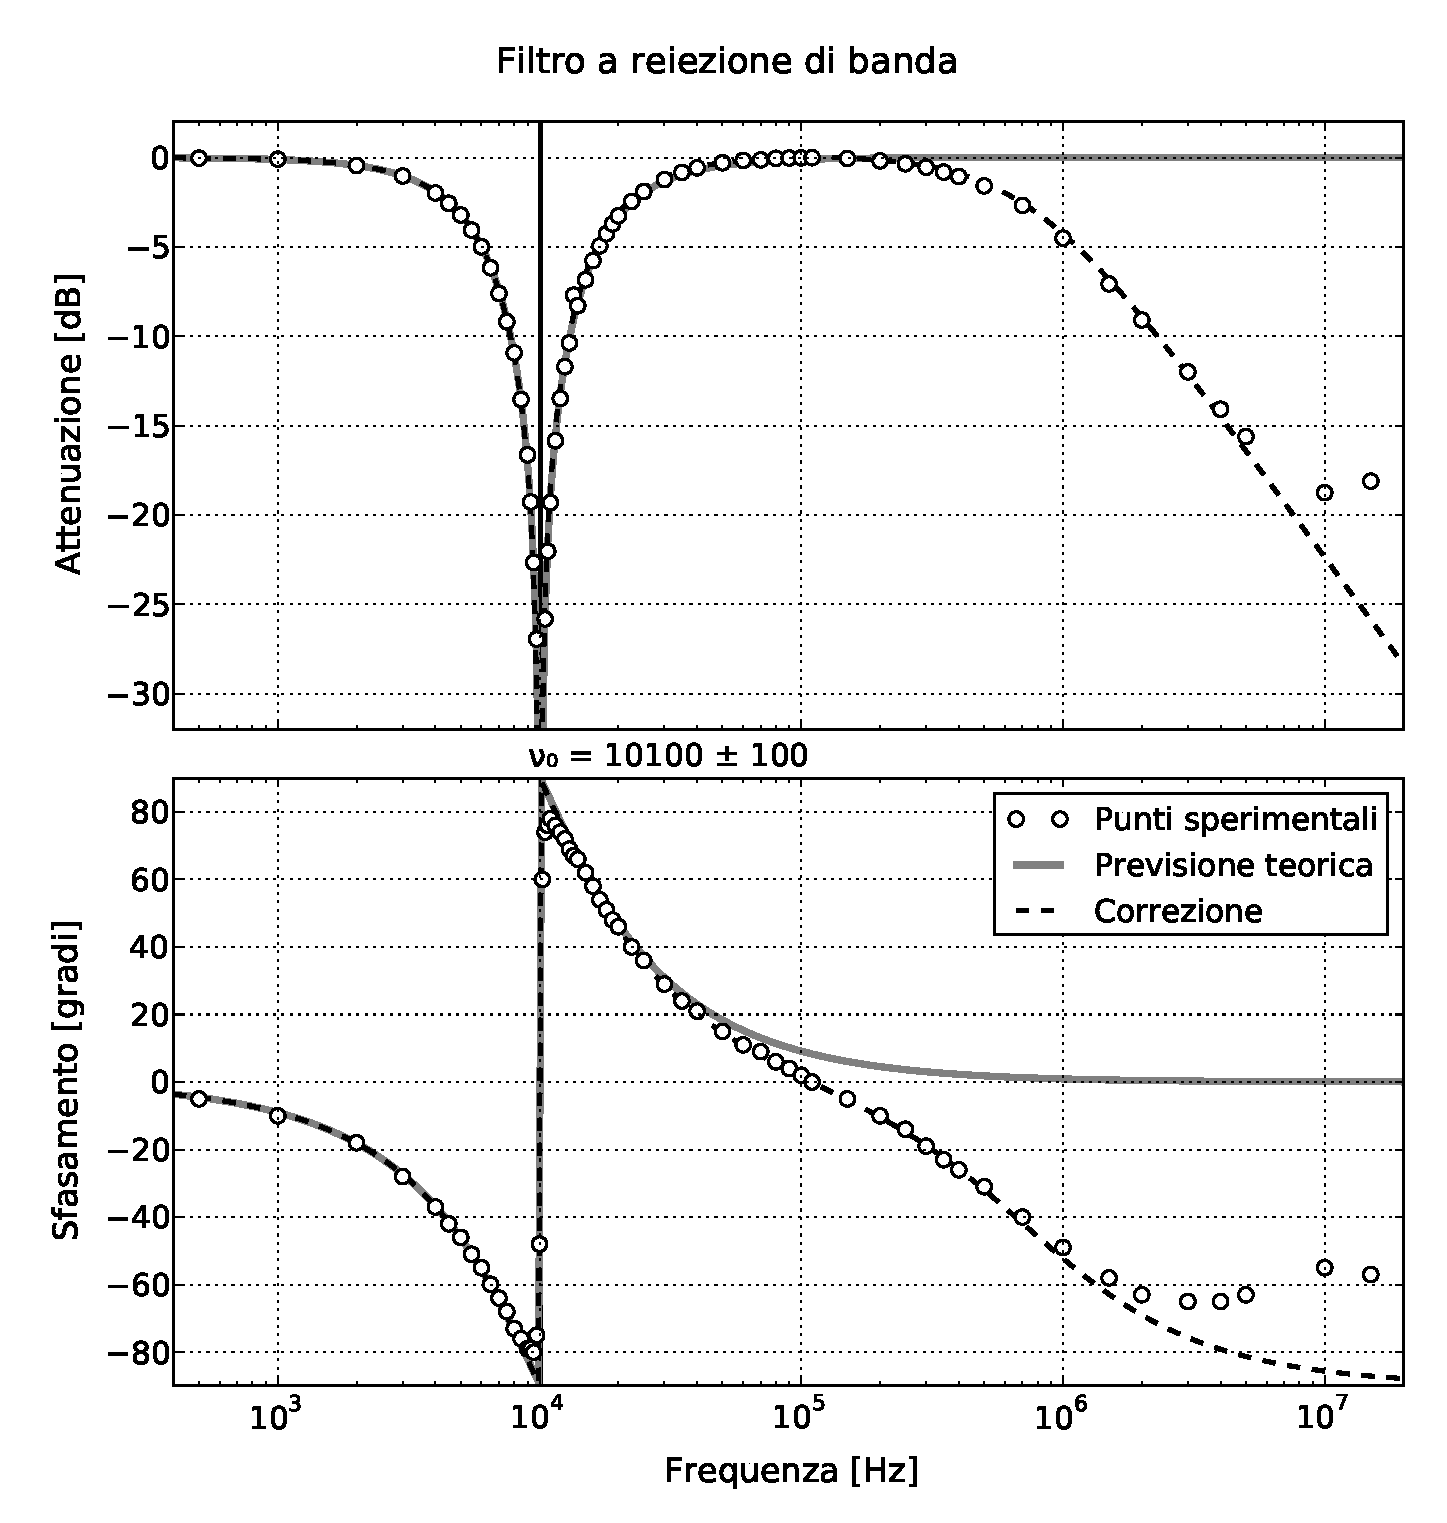
\includegraphics[scale=0.55]{notch.pdf}
  \caption{In questo caso abbiamo
    misurato la risposta del filtro fino a frequenze di 15 Mhz. La predizione teorica, indicata dalla linea
    continua grigia, è in accordo con i dati fino a circa 100 kHz ed in seguito si discosta significativamente
    dal funzionamento reale del filtro. Questo è dovuto al fatto che ad alte frequenze la resistenza dei cavi
    di collegamento inizia a diventare non trascurabile, e insorgono capacità ed induttanze parassite. La linea
    tratteggiata indica una correzione teorica ottenuta considerando una capacità parassita
    $F = 2.1 \times 10^{-10} \si{\farad}$ in parallelo all'induttore, come mostrato in Figura \ref{fig:corr}.
    L'introduzione della correzione spiega molto meglio i dati ottenuti dopo i 100 kHz. Attorno ai 10 Mhz anche la
    correzione inizia a non essere molto aderente alla realtà, a causa del fatto che anche l'effetto delle resistenze
    ed induttanze parassite inizia a farsi sentire.}
  \label{fig:g_notch}
\end{SCfigure}
